% Structure-based materials informatics workflow
% Inspired by fig. 1 in https://doi.org/10.1016/j.cpc.2019.106949.

\documentclass[tikz]{standalone}

\usetikzlibrary{positioning, arrows.meta, calc}

\begin{document}
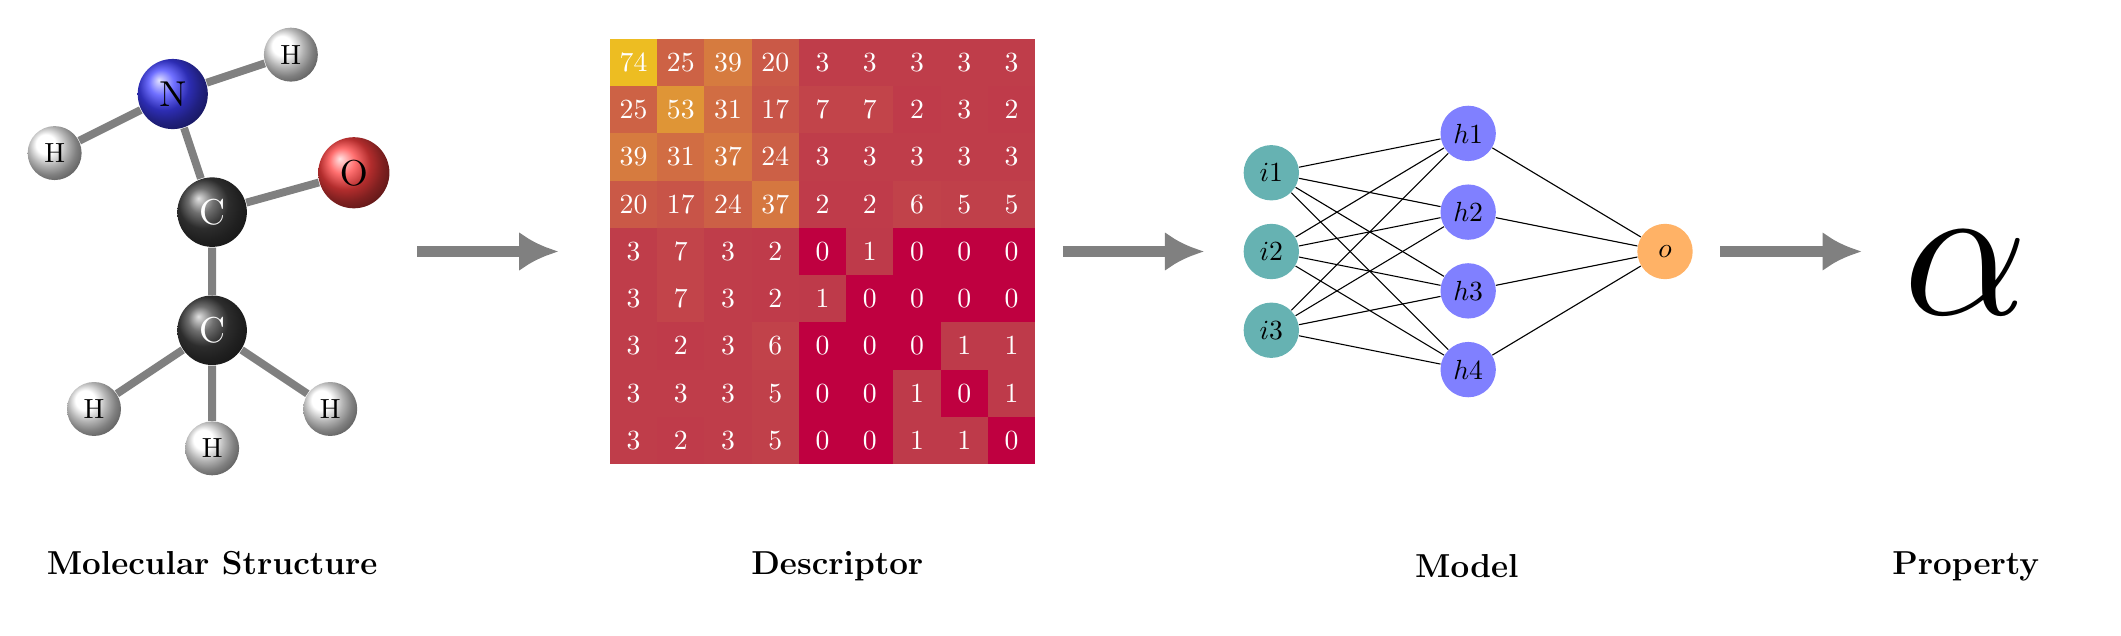
\begin{tikzpicture}[
  neuron/.style={circle,fill=black!25,minimum size=20,inner sep=0},
  label/.style={font=\large\bfseries, minimum size=3em},
  arrow/.style={>={LaTeX[width=5mm,length=5mm]}, ->, line width=1ex, gray, shorten <=1em, shorten >=1em},
  ]


  \begin{scope}[local bounding box=struc]
    \node[ball color=black!75, circle, white, scale=1.3] (C1) at (0, 0) {C};
    \node[ball color=black!75, circle, white, scale=1.3] (C2) at (0, -1.5) {C};
    \node[ball color=blue!75, circle, scale=1.3] (N1) at (-0.5, 1.5) {N};
    \node[ball color=red!75, circle, scale=1.3] (O1) at (1.8, 0.5) {O};
    \node[ball color=white, circle] (H1) at (1.5, -2.5) {H};
    \node[ball color=white, circle] (H2) at (0, -3) {H};
    \node[ball color=white, circle] (H3) at (-1.5, -2.5) {H};
    \node[ball color=white, circle] (H4) at (-2, 0.75) {H};
    \node[ball color=white, circle] (H5) at (1, 2) {H};
    \draw[gray, line width=1mm] (H1) -- (C2) -- (C1) -- (N1) (C1) -- (O1) (H2) -- (C2) (H3) -- (C2) (N1) -- (H4) (N1) -- (H5);
  \end{scope}

  % \draw[rounded corners=1em, thick] (current bounding box.south west)++(-1,-1) rectangle (current bounding box.north east);

  \node[label] at (0,-4.5) (structure) {Molecular Structure\vphantom{p}};
  \node[label, right=4.5cm of structure] (descriptor) {Descriptor};
  \node[label, right=6cm of descriptor] (model) {Model};
  \node[label, right=4.5cm of model] (property) {Property};
  \node[scale=7, above=1.8cm of property] (alpha) {$\alpha$};


  \begin{scope}[shift={($(struc.east)+(2.5,0)$)}, scale=0.6, local bounding box=desc]
    \foreach \y [count=\n] in {
        {74,25,39,20,3,3,3,3,3},
        {25,53,31,17,7,7,2,3,2},
        {39,31,37,24,3,3,3,3,3},
        {20,17,24,37,2,2,6,5,5},
        {3,7,3,2,0,1,0,0,0},
        {3,7,3,2,1,0,0,0,0},
        {3,2,3,6,0,0,0,1,1},
        {3,3,3,5,0,0,1,0,1},
        {3,2,3,5,0,0,1,1,0},
      } {
        \foreach \x [count=\m] in \y {
          \node[fill=yellow!\x!purple, minimum size=6mm, text=white] at (\m,5-\n) {\x};
        }
      }
  \end{scope}

  \begin{scope}[shift={($(desc.east)+(3,2.5)$)}, local bounding box=mod]
    \def\layersep{2.5}

    % Input layer
    \foreach \y in {1,2,3}
    \node[neuron, fill=teal!60] (i\y) at (0,-\y-0.5) {$i\y$};

    % Hidden layer
    \foreach \y in {1,...,4}
    \path node[neuron, fill=blue!50] (h\y) at (\layersep,-\y) {$h\y$};

    % Output node
    \node[neuron, fill=orange!60] (o) at (2*\layersep,-2.5) {$o$};

    % Connect every node in the input layer with every node in the hidden layer.
    \foreach \source in {1,2,3}
    \foreach \dest in {1,...,4}
    \path (i\source) edge (h\dest);

    % Connect every node in the hidden layer with the output layer
    \foreach \source in {1,...,4}
    \path (h\source) edge (o);
  \end{scope}

  \draw[arrow] (struc.east) -- ++(2.5,0);
  \draw[arrow] (desc.east) -- ++(2.5,0);
  \draw[arrow] (mod.east) -- ++(2.5,0);

\end{tikzpicture}
\end{document}